\subsection{Afstandssensor}

\begin{figure}[h]
	\centering
	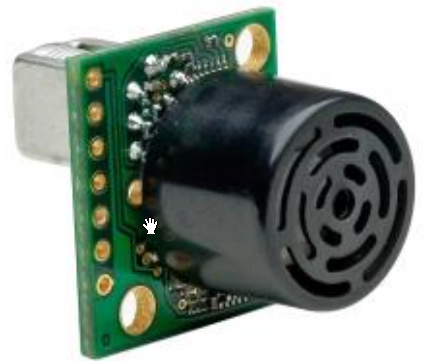
\includegraphics[scale=0.4]{../fig/billeder/distancesensor.png}
	\caption{Afstandssensor MaxSonar1202}
	\label{fig:ds_pic}
\end{figure}

Afstandssensorerne er tilføjet systemet for at kunne videregive data til AKS-klassen så denne kan tage de nødvendige forholdsregler. 
Det er valgt at benytte ultralydssensorer af type MaxSonar1202-typen \cite{lib:maxsonar} til formålet. 
Disse levede op til de stillede krav til systemet om rækkevidde, interface og kommunikationsprotokol.
På sensorprintet var der ydermere mulighed for at tilgå status-pin og alt.-adresse pin. 
Dette blev dog ikke benytte i projektet og der er derfor ikke gjort brug af disse features.

De fire sensorer er montering parvis for og bag på bilen, på figur \ref{fig:ds_mont} ses sensorerne ''Front Left'' og ''Front Right''. 
Overvejelserne i forhold til placering af sensorerne, er taget på baggrund af databladets oplysninger om spredning på scannings-området, og det var vigtigt også at tage højde for rækkevidden der afhænger af den forsyning som sensorerne kører på. 
I placering af sensorerne blev blindvinkelen taget i betragtning, således var det vigtigt for systemet at sensorerne rækkeviddes er placeret så de kan detektere forhindringer også midt for bilen. 
Der blev testet med flere placering af sensorerne, og den endelige placering ses på figur \ref{fig:ds_mont}.  


\begin{figure}[ht]
	\centering
	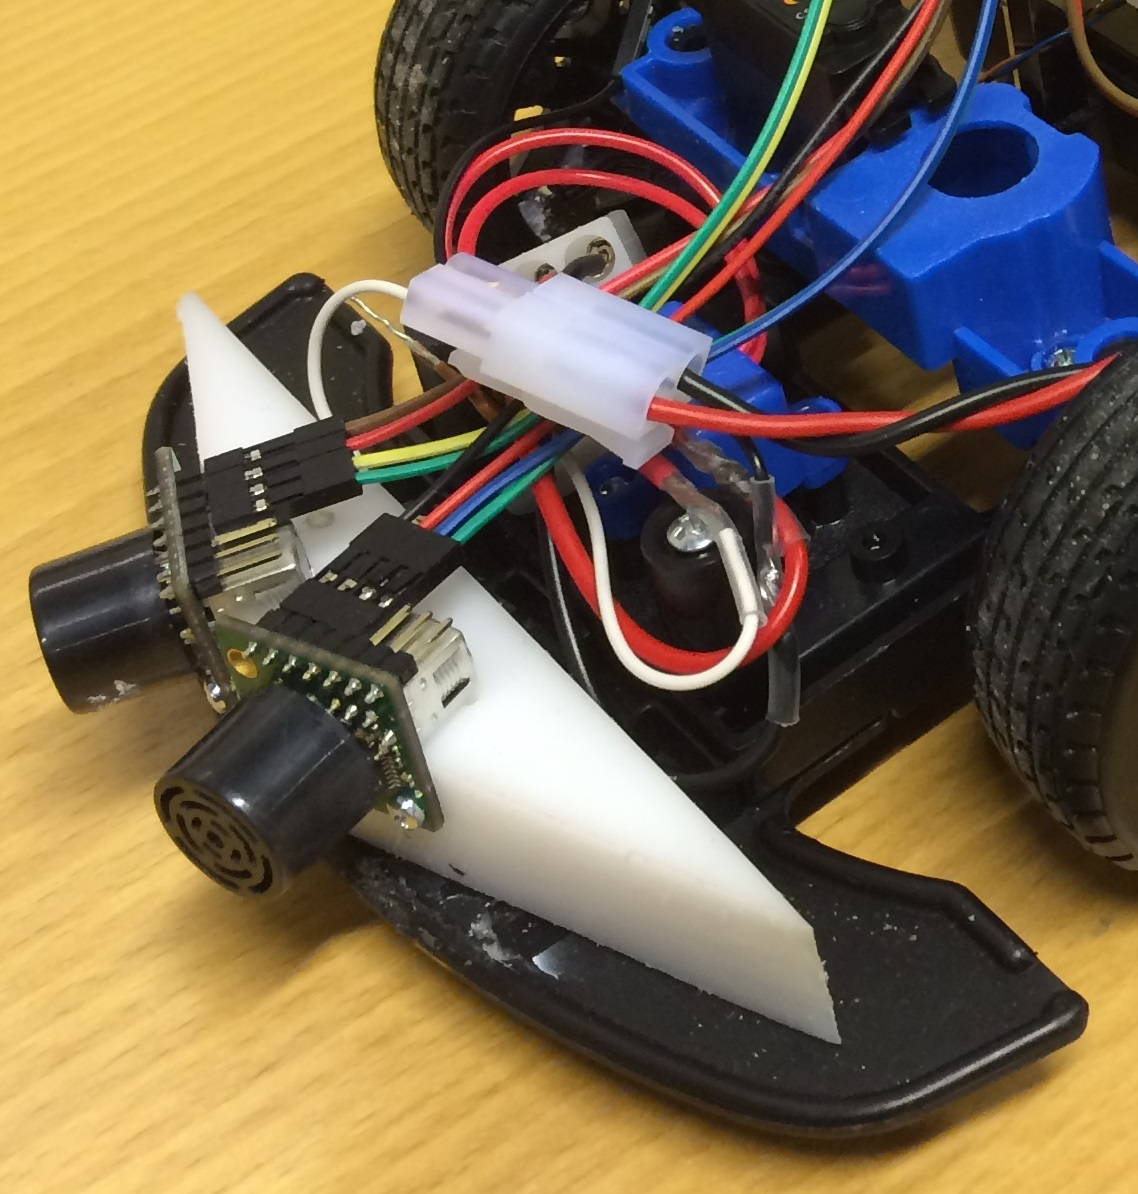
\includegraphics[scale=0.1]{../fig/billeder/distancesensor_montering.jpg}
	\caption{Afstandssensorer monteret på forenden af AU2}
	\label{fig:ds_mont}
\end{figure}

De fire sensorer sidder på fælles \IIC bus med pull-up resistor på datalinjen (\texttt{SDA}) og clocken (\texttt{SCL}). 
Denne del af bussen har PSoC'en som Master og sensorerne som slaver.
I første iteration var det planglagt at sensorerne skulle kommunikere direkte med Pi'en over \IIC-bussen. 
Under implementeringen viste det sig dog ikke muligt at opnå den ønskede kommunikation med Pi'en grundet den kombinerede read/write-struktur i komminukationen med sensorne, for flere detaljer herom hensvises til afsnit \ref{P-sec:hw_design_distancesensor} \nameref{P-sec:hw_design_distancesensor} på side \pageref{P-sec:hw_design_distancesensor} i dokumentationen. 
På baggrund af disse udfordringer er blev det valgt at inddrage PSoC'en i designet som kombineret Master/Slave-enhed og lade denne tage sig af alle sensorer, dette gav en udover at løse \IIC-problematikken og Pi'en mere overskud til at foretage den egne processor.